\documentclass[12pt]{article}%
\usepackage{amsfonts}
\usepackage{fancyhdr}
\usepackage{comment}
\usepackage[a4paper, top=2.5cm, bottom=2.5cm, left=2.2cm, right=2.2cm]%
{geometry}
\usepackage{times}
\usepackage{amsmath}
\usepackage{changepage}
\usepackage{amssymb}
\usepackage{graphicx}

\setcounter{MaxMatrixCols}{30}
\newtheorem{theorem}{Theorem}
\newtheorem{acknowledgement}[theorem]{Acknowledgement}
\newtheorem{algorithm}[theorem]{Algorithm}
\newtheorem{axiom}{Axiom}
\newtheorem{case}[theorem]{Case}
\newtheorem{claim}[theorem]{Claim}
\newtheorem{conclusion}[theorem]{Conclusion}
\newtheorem{condition}[theorem]{Condition}
\newtheorem{conjecture}[theorem]{Conjecture}
\newtheorem{corollary}[theorem]{Corollary}
\newtheorem{criterion}[theorem]{Criterion}
\newtheorem{definition}[theorem]{Definition}
\newtheorem{example}[theorem]{Example}
\newtheorem{exercise}[theorem]{Exercise}
\newtheorem{lemma}[theorem]{Lemma}
\newtheorem{notation}[theorem]{Notation}
\newtheorem{problem}[theorem]{Problem}
\newtheorem{proposition}[theorem]{Proposition}
\newtheorem{remark}[theorem]{Remark}
\newtheorem{solution}[theorem]{Solution}
\newtheorem{summary}[theorem]{Summary}
\newenvironment{proof}[1][Proof]{\textbf{#1.} }{\ \rule{0.5em}{0.5em}}

\newcommand{\Q}{\mathbb{Q}}
\newcommand{\R}{\mathbb{R}}
\newcommand{\C}{\mathbb{C}}
\newcommand{\Z}{\mathbb{Z}}

%%%%
% ME %
%%%%

\usepackage{listings}
\usepackage{color}
\usepackage{xcolor}
\usepackage{mdframed}

\definecolor{dkgreen}{rgb}{0,0.6,0}
\definecolor{gray}{rgb}{0.5,0.5,0.5}
\definecolor{mauve}{rgb}{0.58,0,0.82}

\lstset{%frame=tb,
language=Matlab,
aboveskip=3mm,
belowskip=3mm,
showstringspaces=false,
columns=flexible,
basicstyle={\small\ttfamily},
numbers=none,
numberstyle=\tiny\color{gray},
keywordstyle=\color{blue},
commentstyle=\color{dkgreen},
stringstyle=\color{mauve},
breaklines=true,
breakatwhitespace=true,
tabsize=3
}

\usepackage{outlines}
\usepackage{enumitem}
%\setenumerate[1]{label=\Roman*.}
%\setenumerate[2]{label=\Alph*.}
%\setenumerate[3]{label=\roman*.}
%\setenumerate[4]{label=\alph*.}

\usepackage{titlesec} 

\titleformat{\subsection}[runin]
  {\normalfont\large\bfseries}{\thesubsection}{1em}{}
\titleformat{\subsubsection}[runin]
  {\normalfont\normalsize\bfseries}{\thesubsubsection}{1em}{}

% for enumerate spacing
\newenvironment{tight_enum}{
\begin{enumerate}[label=\alph*.]
\setlength{\itemsep}{0pt}
\setlength{\parskip}{0pt}
}{\end{enumerate}}

\usepackage{exercise}

\setlength\parindent{0pt}

\newcommand{\code}[1]{\texttt{#1}}
\newcommand{\shp}{$>>>$ }
\newcommand{\tab}{\hspace*{45pt}}

\usepackage{multicol}
\setlength{\columnsep}{0.6cm}

\begin{document}

\title{Homework 07: Chapter 10}

\author{EEC 3150}
\date{}

\maketitle

\begin{center}
\fbox{\fbox{\parbox{5.5in}{\centering
For each Python exercise, write a separate Python script. Submit all scripts on Blackboard under the appropriate assignment. Name your script files with the following format: \\
\vspace{10pt}
HW$<$assignment number$>$\_Ex$<$exercise number$>$\_$<$FirstInitial$><$LastName$>$.py \\
\vspace{10pt}
Example: HW01\_Ex01\_GWest.py \\
\vspace{10pt}
For short answer or math exercises, either do your work on a sheet of paper and upload a picture of it to Blackboard or submit some kind of text file or Word document to Blackboard. You can place all such exercises in a single document as long as you clearly label each exercise. These files should follow a similar naming convention as the Python scripts.
}}}
\end{center}


\pagebreak


\begin{multicols*}{2}

%%% NEW EXERCISE %%%
\begin{Exercise}[origin={40 points, Python}]

Create a class Complex which implements complex number arithmetic:

\begin{enumerate}[leftmargin=*]
	\item The class should have two attributes:
	\begin{itemize}[leftmargin=*]
		\item \code{r} (real part)
		\item \code{i} (imaginary part)
	\end{itemize}
	\item The class should have these magic methods:
	\begin{itemize}[leftmargin=*]
		\item \code{\_\_str\_\_} should return a string in the following format \code{a+bi} \\
		1) make sure that if \code{b} is negative, it doesn't print \code{a+-bi} \\
		2) if either \code{a,b} are 0, don't print \code{0+bi} or \code{a+0i}, only print \code{0} if both \code{a,b} are 0 (you'll need some nested \code{if}'s in your method
		\item \code{\_\_add\_\_} should return a new Complex object that is the sum of the two operands
		\item \code{\_\_sub\_\_} should return a new Complex object that is the difference of the two operands
		\item \code{\_\_mul\_\_} should return a new Complex object that is the product of the two operands
		\item \code{\_\_truediv\_\_} should return a new Complex object that is the quotient of the two operands
		\item \code{\_\_neg\_\_} should return the negative of the complex number
		\item \code{\_\_eq\_\_} should return whether two complex numbers are equal
		\item \code{\_\_ne\_\_} should return whether two complex numbers are not equal
	\end{itemize}
	\item The class should have two additional methods:
	\begin{itemize}
		\item \code{conj} (complex conjugate)
		\item \code{mag} (the megnitude of the complex number via the Pythagorean Theorem)
	\end{itemize}
\end{enumerate}

%\rule[0pt]{\linewidth}{1pt}

%\vspace{10pt}

\vfill\null
\columnbreak

For reference, here are some definitions for copmlex arithmetic. Let $x = a + bi$ and $y = c + di$ be two complex numbers. \\

The sum of $x$ and $y$ is:
\begin{align*}
x + y &= (a + bi) + (c + di) \\
      &= (a + c) + (b + d)i
\end{align*}

The difference of $x$ and $y$ is:
\begin{align*}
x - y &= (a + bi) - (c + di) \\
      &= (a - c) + (b - d)i
\end{align*}

The product of $x$ and $y$ is:
\begin{align*}
xy &= (a + bi) (c + di) \\
   &= (ac - bd) + (ad + bc)i
\end{align*}

The quotient of $x$ and $y$ is:
\begin{align*}
\frac{x}{y} &= \frac{a + bi}{c + di} \\
            &= \frac{(ac + bd)}{c^2 + d^2} + \frac{(bc - ad)}{c^2 + d^2}i
\end{align*}

%\rule[0pt]{\linewidth}{1pt}

\vspace{8pt}

Here's some examples of the class and methods: \\

\begin{minipage}{0.7\columnwidth}
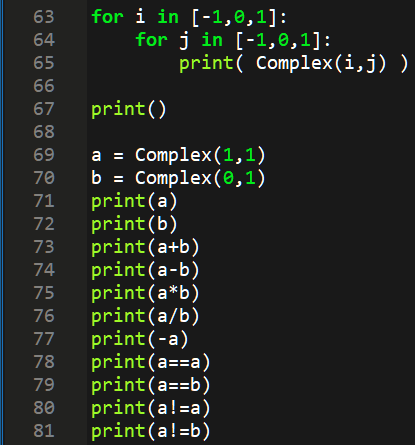
\includegraphics[width=\linewidth]{ComplexTest}
\end{minipage}
\begin{minipage}{0.3\columnwidth}
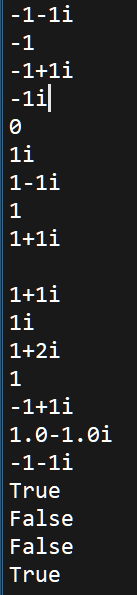
\includegraphics[width=0.6\linewidth]{ComplexResults}
\end{minipage}




\end{Exercise}


\vfill\null
\end{multicols*}




\end{document}






